%\documentclass{article}
\documentclass[12pt,twoside,openright]{report}

%% Useful packages
\usepackage[a4paper,top=1.46in,bottom=1.4in,left=1.46in,right=1.46in]{geometry}
\usepackage{amsmath}
\usepackage{amssymb}
\usepackage{caption}
\usepackage{graphicx}
\usepackage[colorinlistoftodos]{todonotes}
\usepackage[colorlinks=true, allcolors=black]{hyperref}
\usepackage{float}
\usepackage{setspace}
\usepackage{subfigure}
\usepackage{url}
\usepackage{tabularx}
\usepackage[utf8]{inputenc}
\usepackage{mathptmx} %Times Font
\usepackage{titlesec}
\titlespacing{\chapter}{0pt}{0pt}{0pt}
\usepackage{fancyhdr}
\usepackage{etoolbox}
\usepackage{appendix}
\usepackage{gensymb}
\usepackage{siunitx}
\usepackage{nomencl}
\newcommand{\nomunit}[1]{%
\renewcommand{\nomentryend}{\hspace*{\fill}#1}}
\makenomenclature
\usepackage{caption}
\usepackage{lipsum}
\usepackage{algpseudocode}
\usepackage{empheq}
\usepackage{mdwlist}
\usepackage{booktabs}
\usepackage{colortbl}
\widowpenalty 10000
\clubpenalty 10000
\usepackage{moresize}

\usepackage[style=ieee]{biblatex}
\addbibresource{References.bib}
\DeclareSourcemap{
  \maps[datatype=bibtex]{
    \map{
       \step[fieldsource=title, match=\regexp{\b([A-Z]{2,})\b}, replace={{}{$1$}}]
    }
  }
}
 
\DeclareCaptionType{appfigure}[Figure]
\DeclareCaptionType{apptable}[Table]
\renewcommand{\listappfigurename}{List of Appendix Figures}
\renewcommand{\listapptablename}{List of Appendix Tables}
\renewcommand{\thefigure}{\thechapter-\arabic{figure}}
\renewcommand{\thetable}{\thechapter-\arabic{table}}
\renewcommand{\theappfigure}{\thechapter-\arabic{appfigure}}
\renewcommand{\theapptable}{\thechapter-\arabic{apptable}}
\renewcommand{\contentsname}{Table of Contents}

\newcommand{\chapname}{Chapter }
 
\titleformat{\chapter}[block]
{\bfseries\LARGE\centering}
{\chapname \thechapter}{1em}{}[\rule{\textwidth}{0.3pt}]

\titleformat{\section}
{\bfseries\large}
{\thesection}{1em}{}

\titleformat{\subsection}
{\normalfont\bfseries}
{\thesubsection}{1em}{}

\titleformat{\subsubsection}
{\normalfont\bfseries}
{\thesubsubsection}{1em}{}

\usepackage{fancyhdr}
\usepackage{multirow}
\usepackage{multicol}

\usepackage{placeins}

\makeatletter
\renewcommand*\env@matrix[1][*\c@MaxMatrixCols c]{%
  \hskip -\arraycolsep
  \let\@ifnextchar\new@ifnextchar
  \array{#1}}
\makeatother

\usepackage{enumitem}

\usepackage{listings}
\usepackage{color}
 
\definecolor{codegreen}{rgb}{0,0.6,0}
\definecolor{codegray}{rgb}{0.5,0.5,0.5}
\definecolor{codepurple}{rgb}{0.58,0,0.82}
\definecolor{backcolour}{rgb}{0.95,0.95,0.95}

\newcommand{\codesize}{\fontsize{10pt}{11pt}\selectfont}

\lstdefinestyle{mystyle}{
    backgroundcolor=\color{backcolour},   
    commentstyle=\color{codegreen},
    keywordstyle=\color{magenta},
    numberstyle=\tiny\color{codegray},
    stringstyle=\color{codepurple},
    basicstyle=\ttfamily\codesize,
    breakatwhitespace=true,         
    breaklines=true,                 
    captionpos=b,                    
    keepspaces=false,                 
    numbers=left,                    
    numbersep=5pt,                  
    showspaces=false,                
    showstringspaces=false,
    showtabs=false,                  
    tabsize=2,
    showlines = true,
    fontadjust = true,
    framexleftmargin = 10 pt,
    resetmargins = true,
    basewidth = 0.5em
}
 
\lstset{style=mystyle}

\makeatletter
\setlength{\@fptop}{0pt}
\makeatother

\setlength{\floatsep}{0pt}

\newenvironment{Figure}
  {\noindent\minipage{\linewidth}}
  {\endminipage}

\setcounter{secnumdepth}{5}

\hyphenpenalty 10000
\usepackage{multicol}

\usepackage{hyperref}

\hypersetup{
    colorlinks=true,
    linkcolor=blue,
    filecolor=magenta,      
    urlcolor=cyan,
    pdftitle={CE6127 Report},
    pdfpagemode=FullScreen,
    }
    
 
%%%%%%%%% MATHEMATICS SHORTHANDS %%%%%%%%%%%%%%%%%%%% 

\newcommand{\C}{\mathbb{C}}
\newcommand{\R}{\mathbb{R}}
\newcommand{\Z}{\mathbb{Z}}
\renewcommand{\d}{\mathrm{d}}
\renewcommand{\bf}[1]{\mathbf{#1}}

\newcommand{\argmax}[1]{\underset {#1}{\operatorname{arg\,max}}}

\newcommand{\kurt}{\mathrm{kurt}}
\newcommand{\round}{\operatorname{round}}

\newcommand{\E}{\operatorname{E}}
\newcommand{\cov}{\operatorname{cov}}
\newcommand{\pcov}{\operatorname{pcov}}

\newcommand*{\vertbar}{\rule[-1ex]{0.5pt}{2.5ex}}
\newcommand*{\horzbar}{\rule[.5ex]{2.5ex}{0.5pt}}

\setlength{\nomlabelwidth}{3cm}
\setlength{\nomitemsep}{-0.5\parsep}

\usepackage{makecell}
\usepackage{emptypage}

\newcolumntype{R}{>{\raggedleft\arraybackslash}X}
\newcolumntype{L}{>{\raggedright\arraybackslash}X}
\newcolumntype{C}{>{\centering\arraybackslash}X}

\usepackage{textcomp}

%
%\usepackage{background}

%\SetBgScale{1}
%\SetBgContents{\parbox{10cm}{%
%  \Huge Draft:  \today\\[14cm]\rotatebox{180}{\Huge Draft:  %\today}}}
%\SetBgColor{gray}
%\SetBgAngle{270}
%\SetBgOpacity{0.1}
%

%%%%%%%%%%%%%%%%%%%%%%%%%%%%%%%%%%%%%%%%%%%%%%%%%%%%%
\begin{document}
\sloppy
%==== FRONT PART====
\begin{titlepage}
\begin{figure}[!t]
\centering

\includegraphics[width = 4.2in]{Title/logo.png}
\caption*{}
\end{figure}

\centering
\LARGE{\textbf{A Tank Game: Reinforcement Learning using Unity ML Agent }}\\[2.5in]

\large{\textbf{Xavier Tan}}\\
\large{\textbf{Xavier002@e.ntu.edu.sg}}\\[1in]

\textbf{School Of Computer Science and Engineering}\\[0.5in]

\textbf{2022}
\newpage
\end{titlepage}

%\begingroup
%\let\cleardoublepage\clearpage
\pagenumbering{roman}
\pagestyle{fancy}
\fancyhf{}
\cfoot{\thepage}
%\endgroup


\tableofcontents
\rhead{Table of Contents}
\newpage


\newpage

\rhead{Chapter \thechapter}

%==== MAIN PART ====
\pagenumbering{arabic}
\lhead{Introduction}
%=== CHAPTER ONE (1) ===
%=== INTRODUCTION ===

\chapter{Introduction}


\section{Objectives}

This project aims to develop a Deep Reinforcement Learning \cite{li2017deep} (DRL) Tank game prototype using Unity3D \cite{isik2018unityrl} environment and editor. The main goal of the game is to have an autonomous agent tank that can destroy incoming enemy units while allowing friendly units into shelter. The agent tank is also known as the \textbf{turret}. In this game, the \textbf{shelter} is equivalent to the agent's position. 

\section{Scope of Work}
The following characteristics are implemented in this prototype game:
\begin{enumerate}
    \item Enemy or Friendly units die instantaneously, within a single shot.
    \item Bullets / Shells travel infinitely fast.
    \item Enemy / Friendly Units will disappear once it reaches the shelter.
    \item Agent Tank will be stationary, and placed in the center of the game.
    \item Enemy and Friendly units will spawn at random locations around the map.
The game ends when agent tank defeats 20 Enemy Tanks or allow 10 Friendly units into shelter. 
\end{enumerate}


\section{Organisation of Report}

This report is organised into 4 chapters. After this chapter, the next chapter will explain the mechanics, dynamics and aesthetics of the game. In Chapter 3, we will discuss about reinforcement learning and the process of tuning its parameters to achieve near optimal performance. Finally, in chapter 4 we conclude the report.



%=== CHAPTER TWO (2) ===

\chapter{MDA}

This chapter discusses the mechanics, dynamics and aesthetics of the game. We refer agent tank to the tank that is stationary in the center of map and it is fully autonomous. To achieve the intelligence for autonomous control, it trains a NN model using reinforcement learning. Further details will be discussed in Chapter 3. 
\FloatBarrier

\label{sec:MDA}

\section{Mechanics}

\subsection{Agent Tank}
The agent tank's actions are controlled autonomously via function approximator (i.e. deep neural network) trained using UnityML's reinforcement learning framework. This framework is implemented using Tensorflow\cite{goldsborough2016tour} and communicates and with unity editor via an API implemented using python. 


The agent has the action to shoot, and rotate about the same position. It does not have the ability to move. The agent tank uses Unity's \textit{RayPerceptionSensor} \cite{majumder2021understanding} module to differentiate the enemy tanks from friendly tanks as they are tagged differently.

\subsection{Enemy AI}
\begin{figure*}[t]
\centering
\begin{multicols}{2}
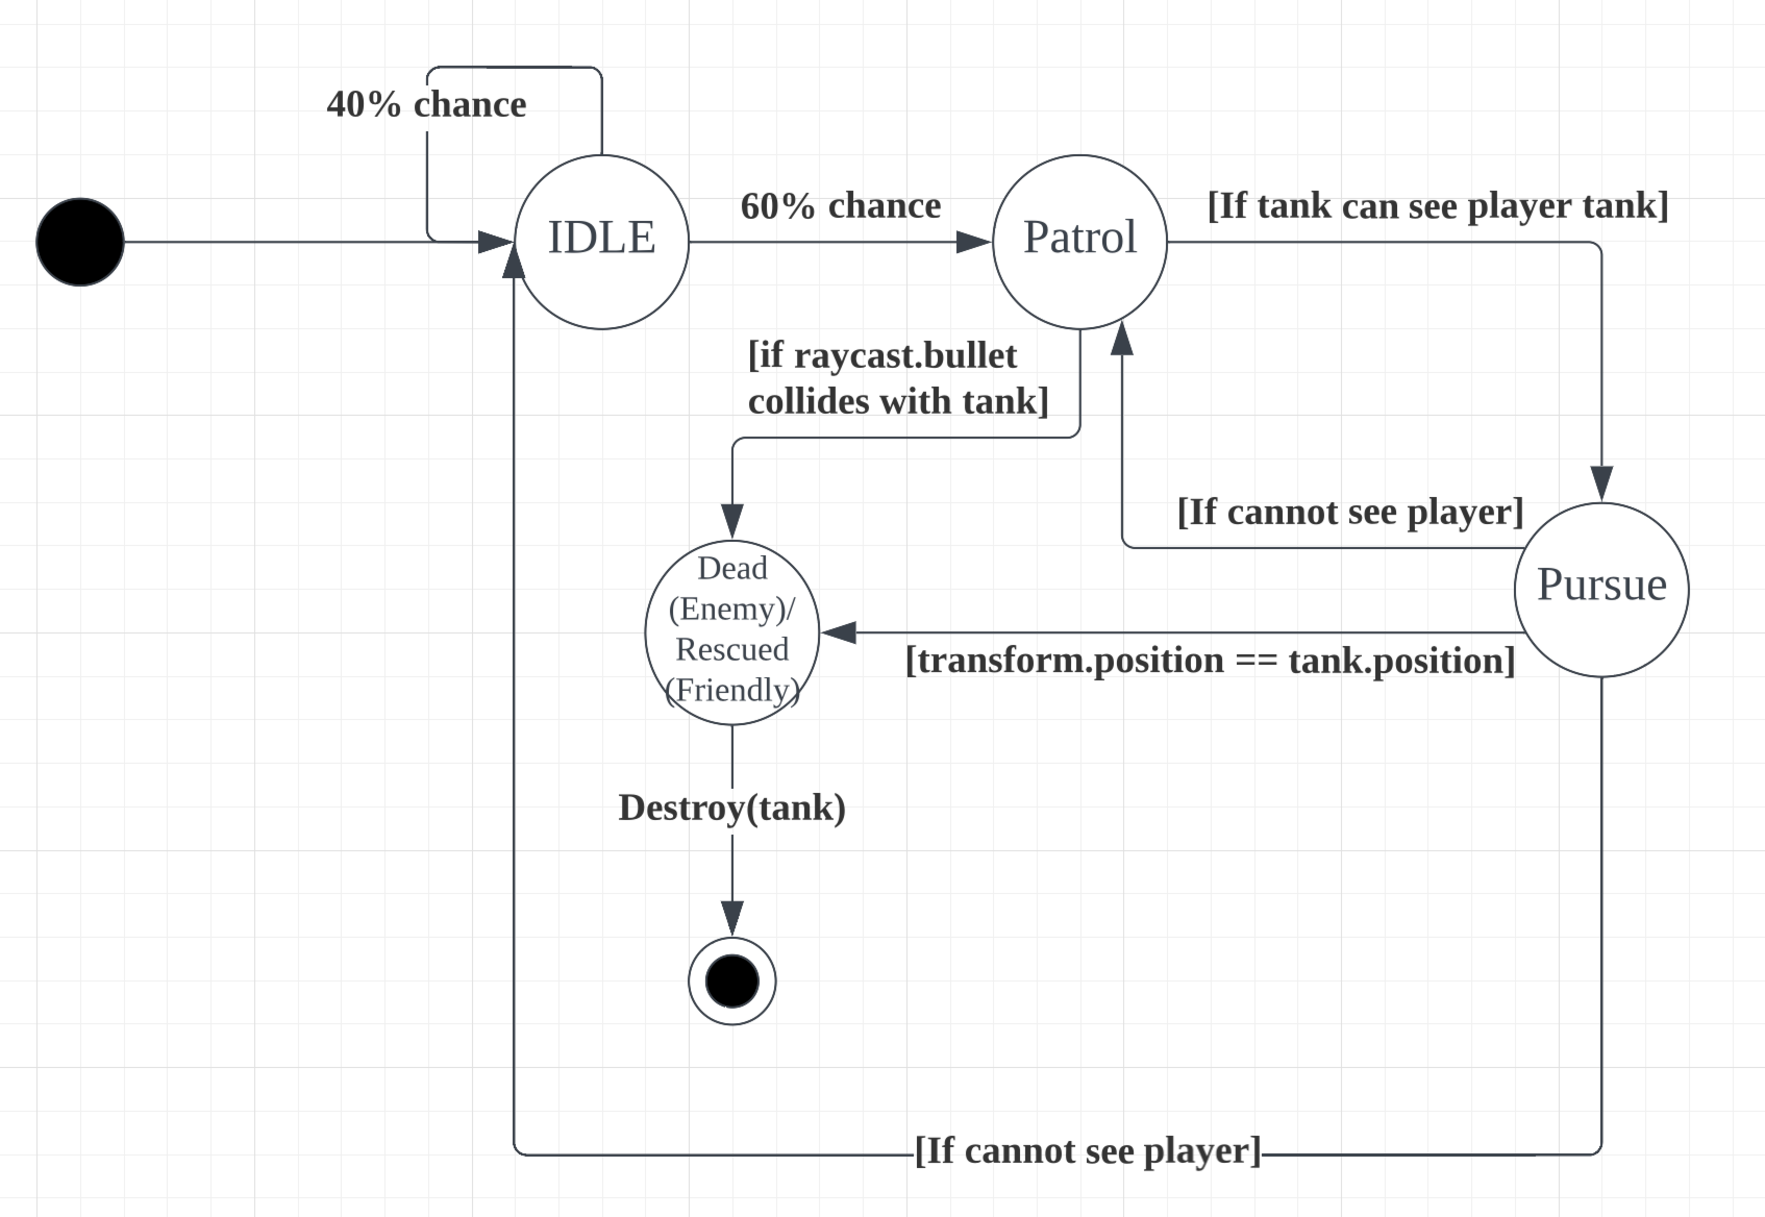
\includegraphics[width=0.99\columnwidth]{Chapter2/Enemy_AI.pdf}
\caption{Finite state machine for enemy and friendly tanks}
\label{fig:FSM_enemy}

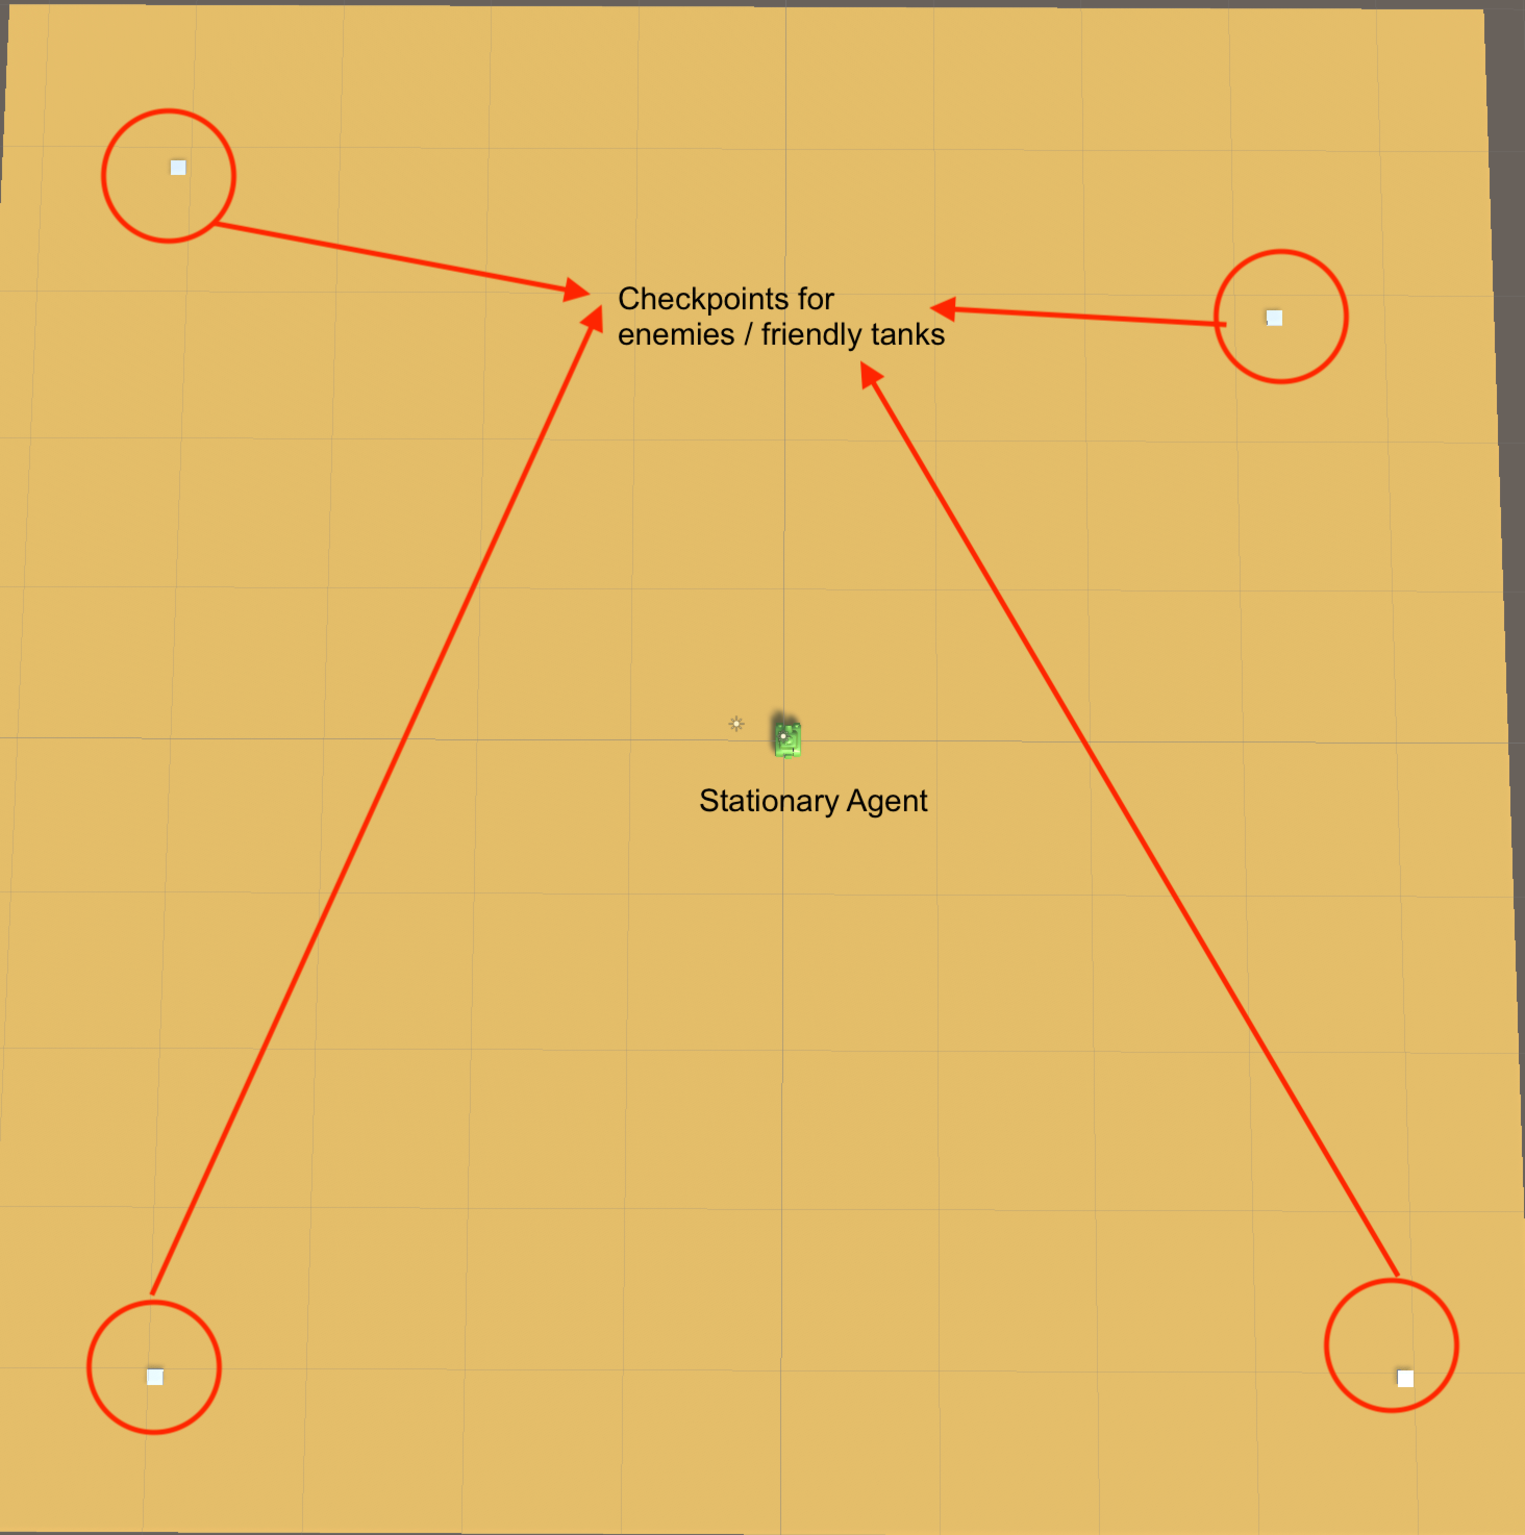
\includegraphics[width=0.99\columnwidth, height=0.7\columnwidth]{Chapter2/Map.pdf}
\caption{Finite state machine for enemy and friendly tanks}
\label{fig:Map}

\end{multicols}
\end{figure*}

The enemy and friendly follows a finite state machine (FSM) as depicted in Figure. \ref{fig:FSM_enemy}. Although both tanks follow the same FSM, the agent differentiates them using Unity's tag system and allocate rewards accordingly.

We used "checkpoints" to guide the enemy tanks in the area where they should patrol. These checkpoints are effectively way-points that are placed in the four corners of the map. This way, the enemy tanks will visit these way-points in an orderly manner, creating the illusion that they are patrolling. Similar to Assignment 1 the \textit{NavMeshAgent} from Unity3D was utilized for enemy and friendly tank’s ability to move around the map. 

\section{Dynamics}

Enemy and Friendly tanks are spawned randomly around the map such that the Agent tank cannot predict where these tanks will spawn over million of rounds of play. To aid the agent tank, bullets travel instantaneously (i.e. using raycasting) hence it does not have to account the travel time of the shell which can be very tricky with simply DRL and no logic coding (i.e. account for when delay in shooting). It is noted that due to the physical size of the tank, a physics \textit{SphereCast} is used instead of \textit{Raycast}. As \textit{Raycast} could miss the tank when the agent tank aims off center of the tank. \textit{SphereCast} allows for more margin of error when aiming at tanks. To ensure fairness, the radius of sphere cast is kept at 1.
However, to prevent the loophole of simply spraying and spamming shells everywhere; without aiming and hoping to hit something. A cool down for shooting a shell is implemented as well as a limit is placed on how fast the agent tank can turn (i.e. maximum of $90\degree / sec $). Conversely, the rewards and penalty given to agent will reflect this idea.

To make things even more interesting, Enemy and Friendly tanks have limited range of detection for agent tank. That is, if they are spawned very far away from agent tank, they would simply patrol around the map until agent tank is within their range. Waypoints are carefully calibrated to ensure that this happens within a single round of patrol, to speed up the game play. Figure. \ref{fig:Map} shows where the waypoints are. Similarly, agent has a limited range of view (i.e. limited rays, angle and distance), as depicted in Figure. \ref{fig:rays}. Such limitation, brings two advantages. 

\textbf{One}, it reduces the chance of clustering, that is when too many enemy and friendly tanks is spawned on the map the agent tank physically do not have enough time to react (due to the imposed limitation). \textbf{Two}, it introduces some form of fairness, otherwise the agent can simply sense all the tanks without even turning.

\section{Aesthetics}

The enemy tanks are the ones in red and purple (Figure. \ref{fig:enemy}) in color. The friendly tanks are in gold color as depicted in Figure. \ref{fig:friendly}. The visuals are different for us human observers to differentiate the tanks and judge the performance of the agent. However, to the agent tank, the tags matters more. As mentioned above, the game is designed to allow as little loophole as possible to maintain certain level of difficulty for the agent as well as a fair environment for the agent to train in. Success can easily be measured if the agent is able to reach the goal by proper means, such as target only enemy tanks and not friendlies. As much as possible, kill enemy tanks while allowing friendlies into the shelter area. Failure can be observed when the agent simply spam shoots and keep turning around, or do nothing and allow anyone to come into its area.

The map is kept relatively simple to allow for effective DRL training. However, later more models such as trees and rocks will be added to increase level of difficulty and test intelligence level of the trained agent tank. An example of this map is shown in Figure. \ref{fig:map_2}.

\begin{figure}
    \centering
    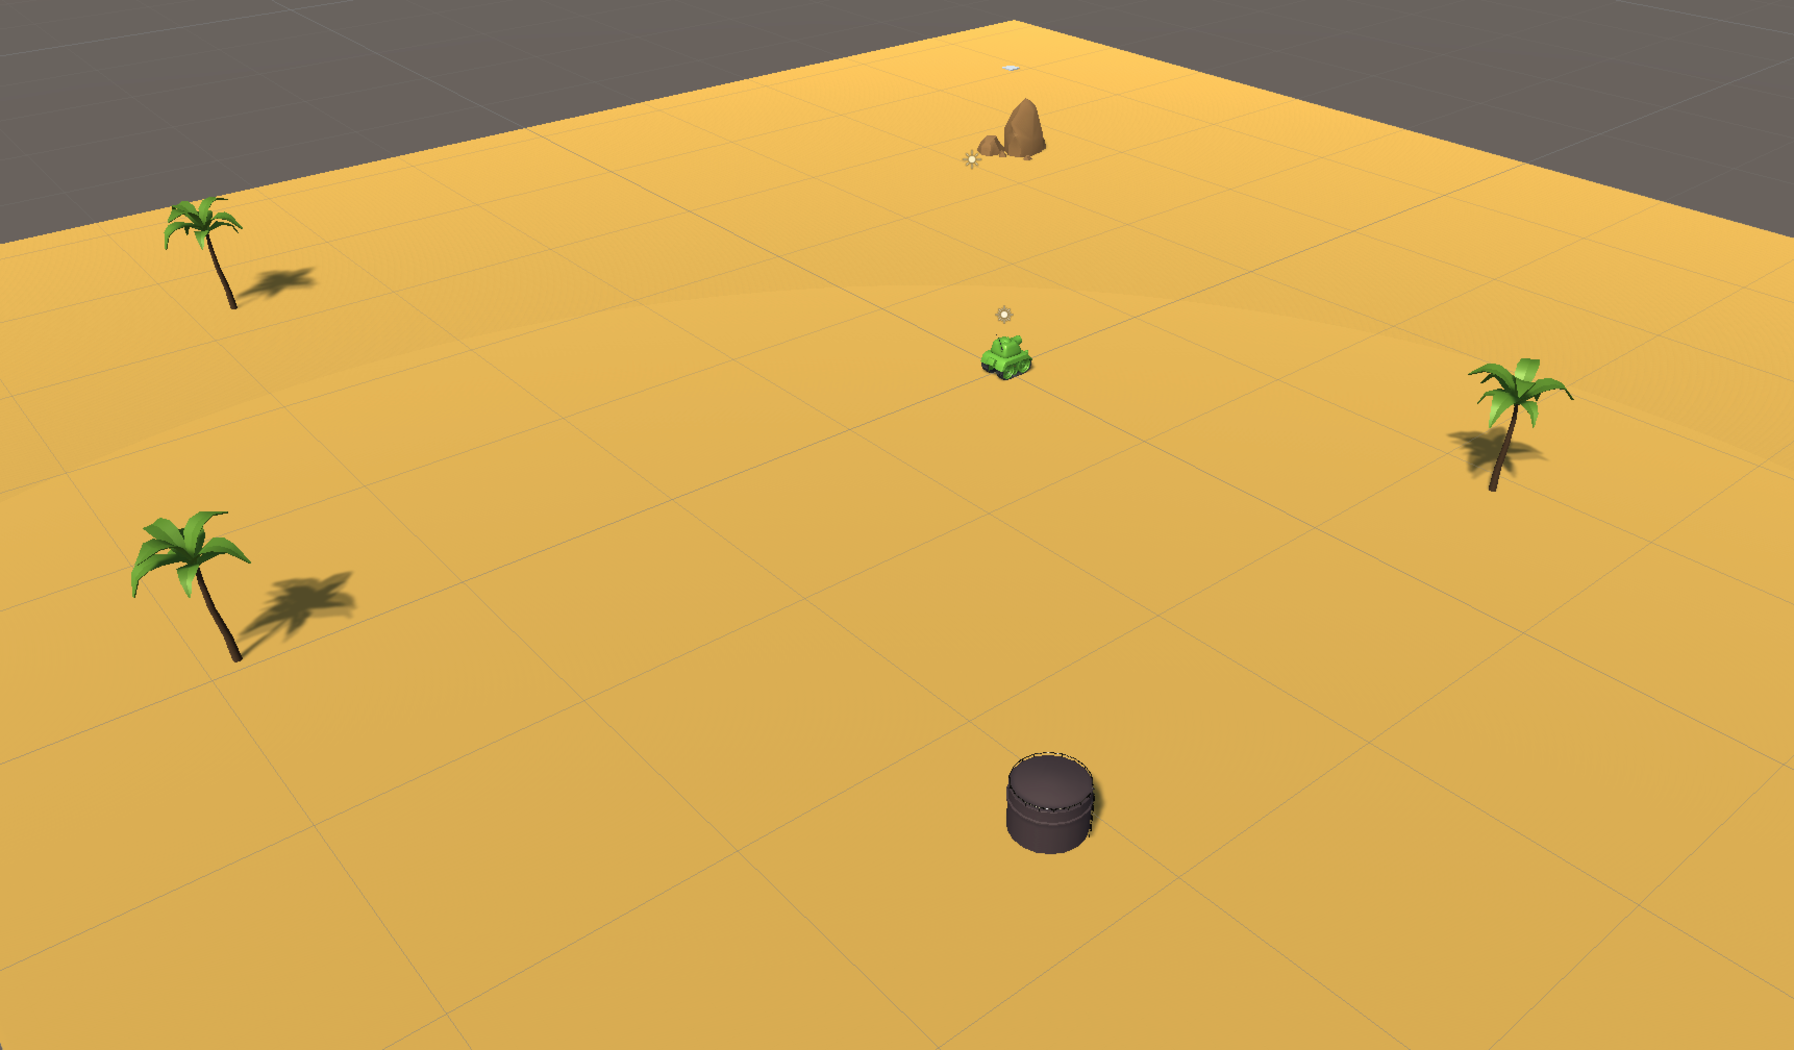
\includegraphics[height=0.5\columnwidth]{Chapter2/Map_2.pdf}\par
    \caption{Map of higher difficulty}
    \label{fig:map_2}
\end{figure}

\begin{figure*}[t]
\centering
\begin{multicols}{3}
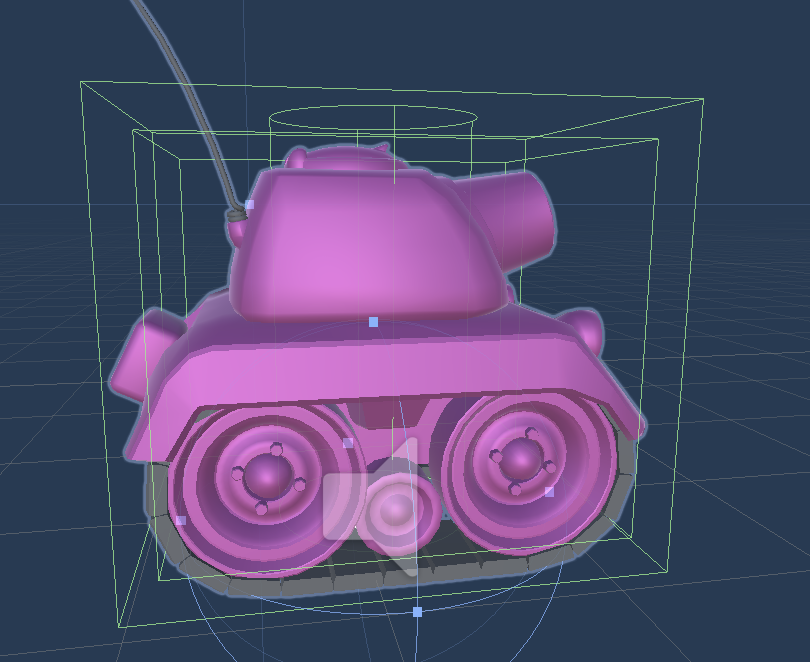
\includegraphics[width=0.99\columnwidth]{Chapter2/enemy_tank.png}\par
\caption{One of the Design of Enemy Tank}
\label{fig:enemy}


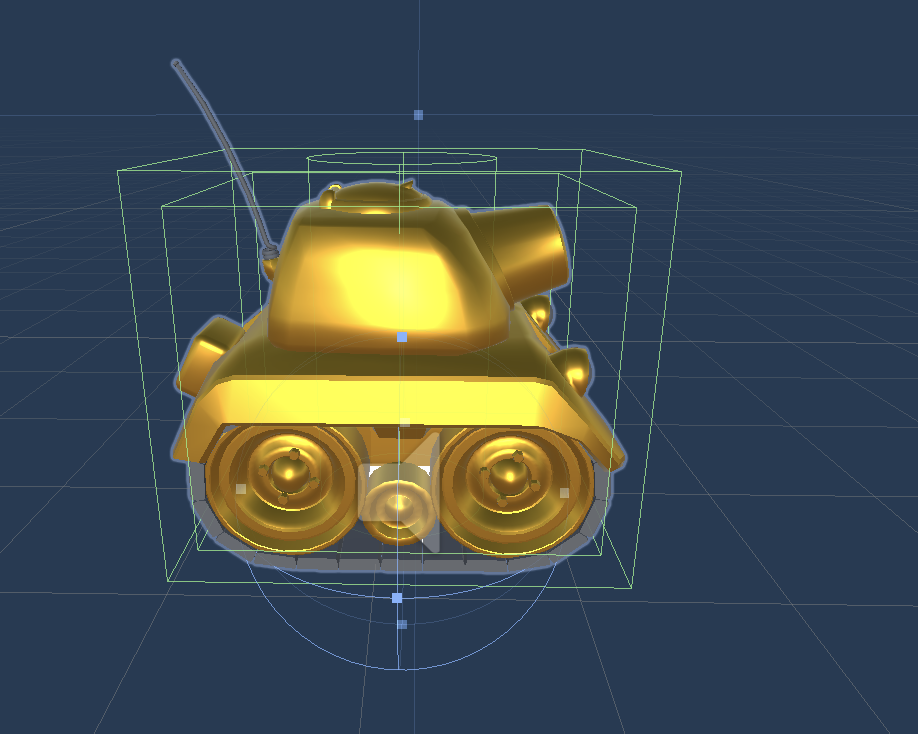
\includegraphics[width=0.99\columnwidth]{Chapter2/friendly_tank.png}\par
\caption{Design of Friendly Tank}
\label{fig:friendly}

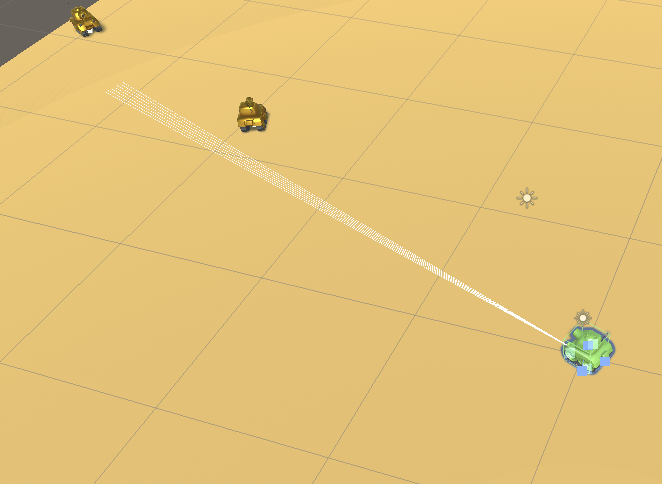
\includegraphics[width=0.99\columnwidth]{Chapter2/Raycast.png}\par
\caption{Agent Tank has limited range of Raycast to balance difficulty}
\label{fig:rays}
\end{multicols}
\end{figure*}

%=== END OF CHAPTER TWO ===


\chapter{Reinforcement Learning}

The details of the experiments and the performance metrics used are discussed in this chapter. The results and discussion are presented here.

\section{Policy}

Two state-of-art deep reinforcement learning algorithms are provided by unityML-Agent API, namely: proximal policy optimization (PPO) \cite{schulman2017proximal} and soft actor critic (SAC) \cite{haarnoja2018soft}. These algorithms utilises a neural network (NN) to approximate the optimal function that maps the agent's observations to the best strategy the agent could take given its current state. Although in complex situation SAC performs much better overall, we chose the PPO algorithm simply because the game environment is relatively simple (i.e. strategy space for agent is not very huge) and cheap to sample (i.e. not much computational resource required to run the game). PPO basically has the objective of optimizing the follow equation:

\begin{equation}
    \mathcal{L}^{clip}(\theta) = \hat{\mathbb{E}_t} \biggr[\min(r_t(\theta)\hat{A}_t, clip(r_t(\theta),1-\epsilon,1+\epsilon)\hat{A}_t)    \biggr],
\end{equation}
where $\theta$ represents the policy parameters, $\hat{A}_t$ denotes the advantage estimate at step $t$, $r_t(\theta) = \frac{\pi_\theta (a_t | s_t)}{ \pi_{\theta_{old}} (a_t | s_t) }$ is the probability ratio of new and old policy (i.e. action $a$ given state $s$ at time step $t$) and $\epsilon$ is a hyperparameter of small value. Clip is the short form for gradient clipping. $\hat{\mathbb{E}_t}[\cdot]$ represents the empirical average over the batches of sample data. Figure \ref{fig:PPO}, depicts the flow diagram for the PPO, actor-critic style algorithm DRL.

\begin{figure}
    \centering
    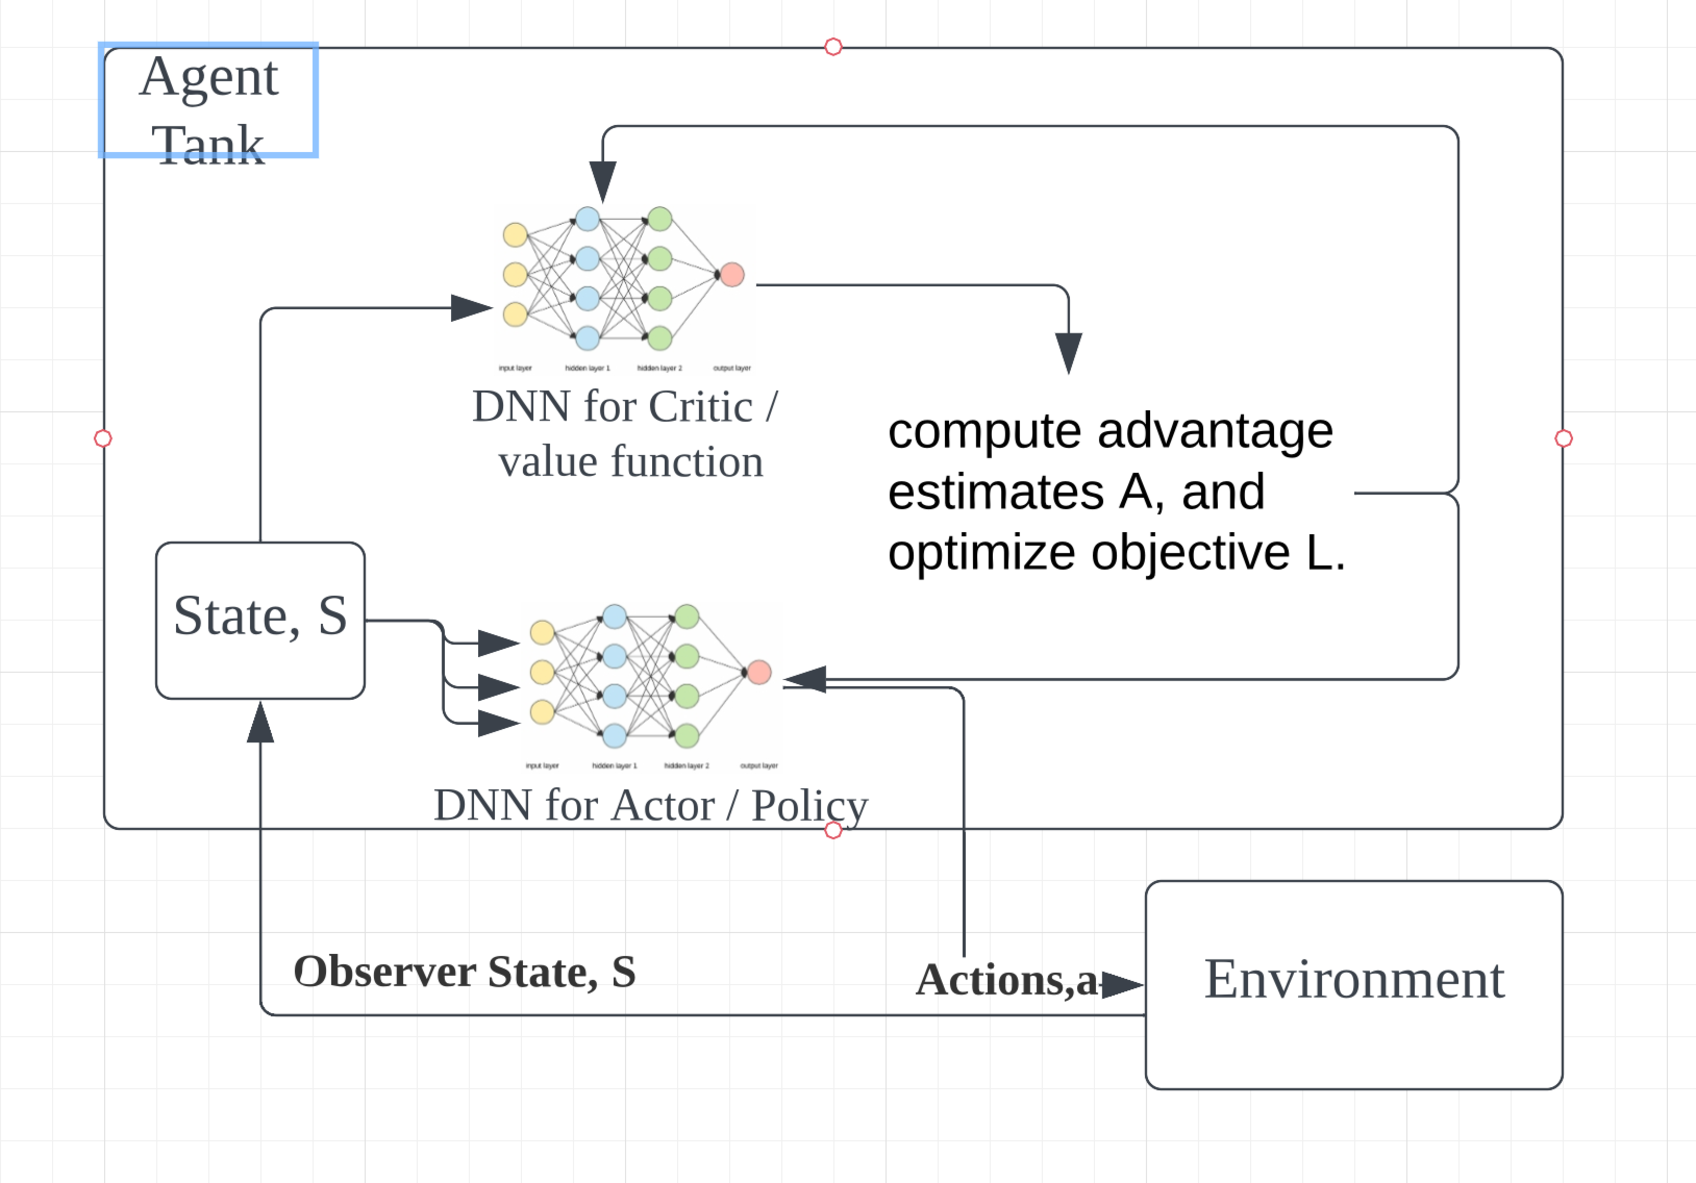
\includegraphics[height=0.6\columnwidth]{Chapter3/PPO.pdf}\par
    \caption{Actor Critic Style PPO}
    \label{fig:PPO}
\end{figure}

\subsection{Observation Possibilities}

The agent can observe the following parameters:
\begin{enumerate}
    \item Agent's current local rotation: A Quarternion
    \item A time: For shooting cooldown
    \item \textit{RaycastSensor} module to act as a laser pointer to sense the different tanks and its position.
\end{enumerate}

The agent has 2 continuous action space (turning clockwise and anticlockwise), and 2 discrete branches, each with 2 action size namely: \textbf{toFire} or \textbf{notFire} and \textbf{canShoot} or \textbf{cannotShoot}. \textbf{canShoot} to shoot means the cool down is over and agent can shoot whenever it requires. \textbf{toFire} is the very action of shooting a shell. This brings the space size for vector observations to 6.

\subsection{Reward and Penalty Rules and corresponding value}
The agent will obtain some positive rewards when:
\begin{enumerate}
    \item Agent destroys an Enemy, 0.5,
    \item Agent allows a Friendly tank to enter shelter area, 0.08,
    \item Agent successfully achieve the goal and end the episode, 1,
\end{enumerate}
The agent will receive some penalty (negative rewards) when:
\begin{enumerate}
    \item Agent allows enemies into the shelter area, -0.8f,
    \item Agent shoots into friendlies, -0.3,
    \item Agent shoots into random, empty area, -0.2,
    \item Agent tries to shoot while reloading, -0.03,
    \item Agent does nothing, -1 / \textit{MaxStep},
\end{enumerate}

It can be noted that the rewards for allowing a friendly tank into shelter area is exceptionally low, compared to other positive actions. This is such that it forces the tank to act and not simply remain nothing. As the tank could win through a loop hole where it simply allow all types of tank to enter the shelter area and win the game when number of friendlies is more than 10, especially when agent tank do not die. This also explains why the penalty for allowing enemy tank into shelter is 10 times that of reward for allowing friendly tank into shelter. Theoretically, a perfect agent can score a maximum of $11 = 0.5*20 + 1$, but this score is likely to be impossible as we have to factor in some enemies inevitably move into the shelter area, and lower rewards for allowing friendly to enter. A more conservative estimate could be that, we take an average for all the rewards, multiply by 20. That is for every enemy destroyed (step closer to winning condition), the agent tank will also take all other actions one time. This method gives us a value of 0.625. In other words, for a agent to work somewhat well, we should expect to see a cumulative reward of above $0.625$.

The penalty for agent doing nothing is encourage the agent to finish the episode quickly, and scales inversely proportional to \textit{MaxStep}, the number of maximum steps the DRL can take. To force the agent to learn that every shot count, because of the cool down for shooting as well as limited turning speeds, a penalty is placed when agent shoots without aiming properly. The other rewards, are given accordingly when agent does something that is favourable to winning the game and given a penalty when it is unfavourable or adds no value to agent's intelligence in winning the game. The game ending is equivalent to ending of one DRL training episode, where the agent will replay the game and strive to do earn higher rewards.


\section{Hyper Parameter tuning}
There are a multitude of parameters that can be tuned to help the agent achieve a better policy in the below section, we will explain each of their significance and justify their values. Table. \ref{tab:sym1} is a summary of the final parameters used to achieve the best agent tank to the best of our ability. Before going into details of the parameter tuning, the metrics used to evaluate parameters will first be explained. The parameters are configured in a YAML \cite{ben2009yaml} file. 

\subsection{Metrics}
\label{Metrics}
%TODO: change langugage

We used Tensorboard to visualise the results of the agent's learning and the graph values have been smoothed out to aid in trend observations.
\subsubsection{Cumulative reward}

Cumulative reward represents the mean cumulative episode reward for all the agents (only one in our case). It should increase when training process is successful. The general trend should show it consistently increase over time. Under complex situations, rewards are not expected until millions of steps into the training process.

\subsubsection{Entropy}
Entropy is used to measure how random the decisions of the model is. It Should slowly decrease when training process is successful. If it decreases too fast, then beta, $\beta$ should be increased.  If it is not decreasing not at all, $\beta$ should be decreased.


\subsubsection{Value loss}
The value loss is the loss in the prediction of the value of each state. 
A lower value loss indicates that the agent makes better predictions. This loss is expected to increase when agent is learning and decrease when the rewards stabilizes.

\subsubsection{Policy loss}

This along with value loss and entropy makes up for all the loss for PPO. It denotes the correlation of how much the policy is changing. The loss magnitude should decrease when a training session is successful.


\subsection{Beta}

The beta, $\beta \in [0.00001, 0.01]$ value denotes the strength of the entropy regularization. 
The larger the value is the more random actions the agent would take, as greater $\beta$ value makes the policy more randomized. Ideally, the optimal $\beta$ value would allow the entropy to slowly decrease as rewards increases. When entropy drops too quickly, $\beta$ has to be increases. Likewise, if entropy decreases too slowly, $\beta$ should be lower. This value would be determined through trial and error as seen in Figure. \ref{fig:beta_entropy}, \ref{fig:beta_cumreward}, \ref{fig:beta_valueLoss}. In all these three metrics, the $\beta$ value of $0.001$ outperforms $\beta$ value of $0.01$. Additionally, we can observe that as cumulative rewards increases, value loss decreases.

\begin{figure*}
\centering
\begin{multicols}{3}
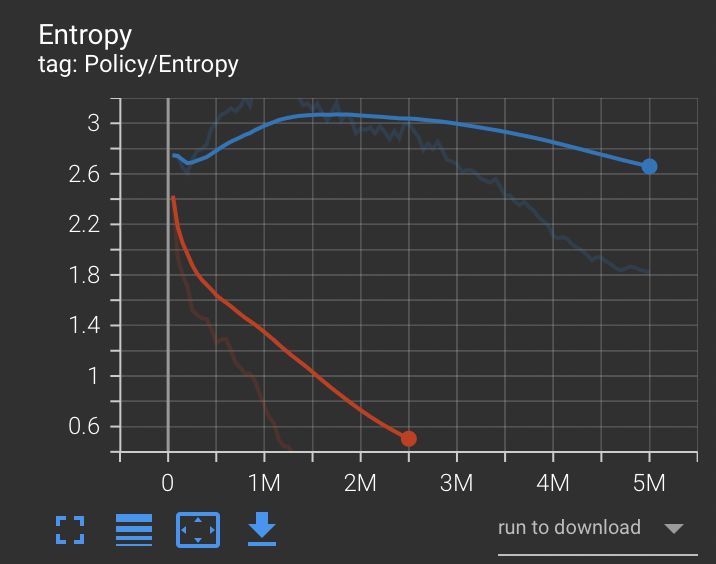
\includegraphics[width=0.99\columnwidth]{Chapter3/beta/beta_entropy.png}\par
\caption{Lower beta of 0.001(red) able to achieve lower entropy than higher beta of 0.01(blue) }
\label{fig:beta_entropy}

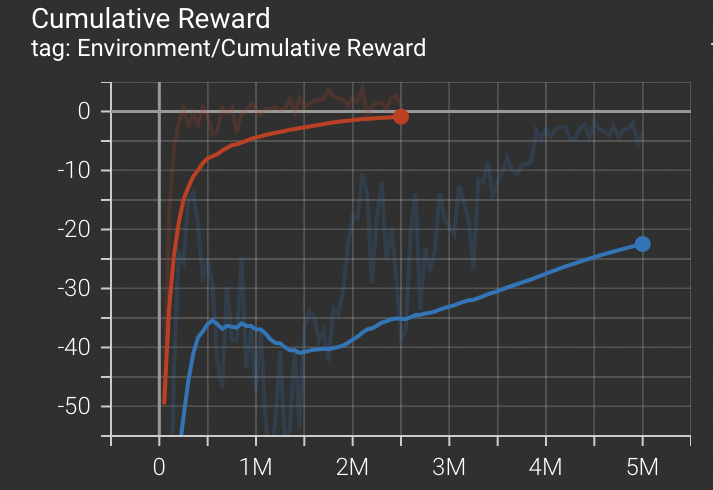
\includegraphics[width=0.99\linewidth]{Chapter3/beta/beta_cumu_reward.png}\par
\caption{Lower beta of 0.001(red) able to achieve higher cumulative external rewards than higher beta of 0.01(blue).}
\label{fig:beta_cumreward}

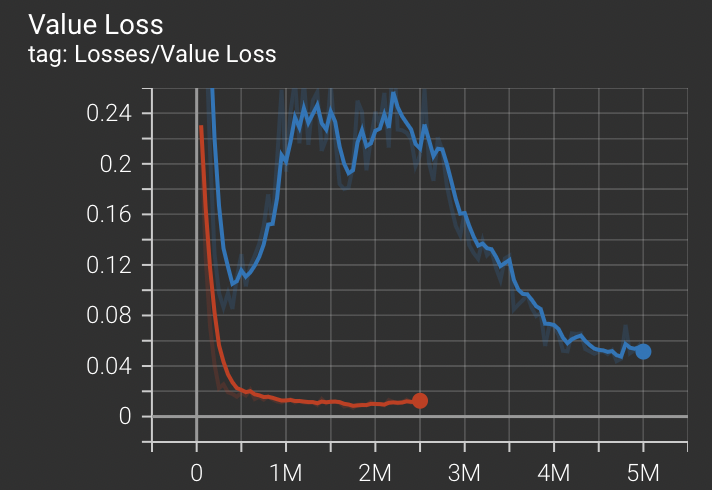
\includegraphics[width=0.99\columnwidth]{Chapter3/beta/beta_value_loss.png}\par
\caption{
Lower beta of 0.001(red) able to achieve lower policy loss than higher beta of 0.01(blue) 
}
\label{fig:beta_valueLoss}
\end{multicols}
\end{figure*}


\subsection{Hidden Units and Layers}
\begin{figure*}
\centering
\begin{multicols}{2}
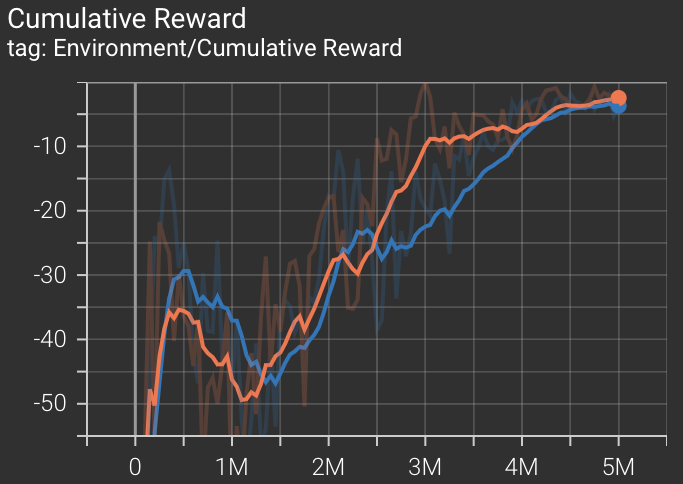
\includegraphics[width=0.99\columnwidth]{Chapter3/HU/cumulative_reward.png}\par
\caption{ $256$ hidden units(blue) able to achieve similar rewards compared to $512$ hidden units (red) }
\label{fig:hu_cumreward}

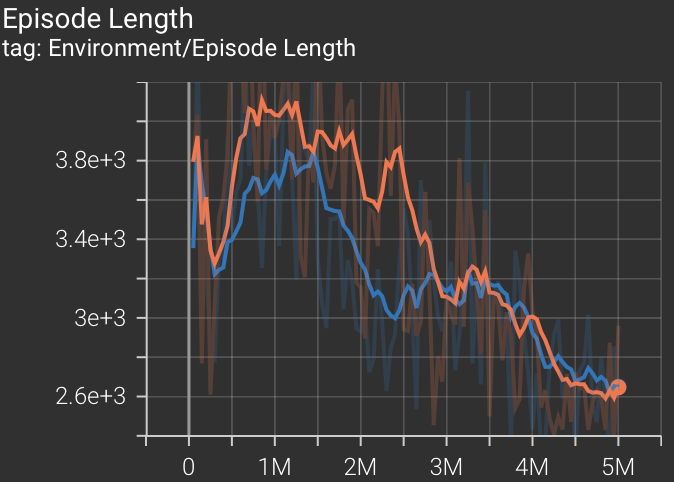
\includegraphics[width=0.99\columnwidth]{Chapter3/HU/episode_length.png}\par
\caption{
$256$ hidden units(blue) able to finish episodes faster than $512$ hidden units (red) 
}
\label{fig:hu_episode}
\end{multicols}
\end{figure*}

We could increase hidden units (HU) and layers to increase capacity of the NN and reduce possibility of under-fitting and over-fitting which result in better approximation. Number of HU ranges between $32$ and $512$ and number of layers ranges between $[1,3]$. The optimal values of these parameters will be approximated through trial and error experimenting. The cumulative rewards achieved by an agent with $256$ and $512$ HU can be observed from Figure. \ref{fig:hu_cumreward}. Both are able to achieve comparable results, yet from \ref{fig:hu_episode} we can observe that the model with $256$ HU is able to finish an episode of training faster than its counterpart. Which means, $256$ HU might be more suitable, especially when our tasks is not as complex.

\begin{figure*}
\centering
\begin{multicols}{2}
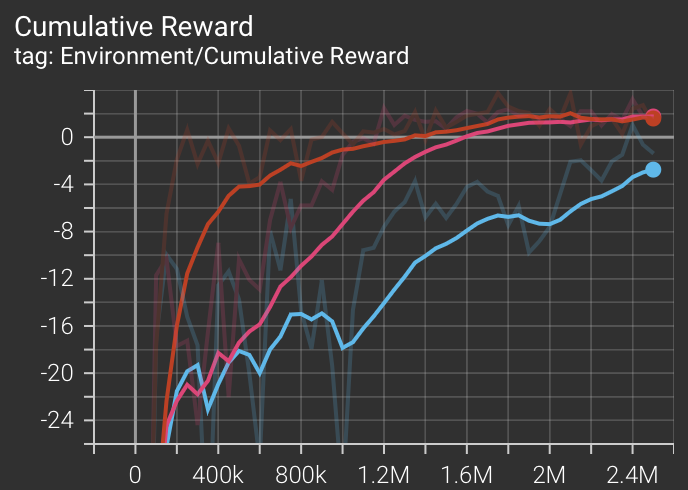
\includegraphics[width=0.99\columnwidth]{Chapter3/HU/layers_cum_reward.png}\par
\caption{ $2$ layers (red) outperforms $3$ layers (blue) and $1$ layer (pink)}
\label{fig:la_cumreward}

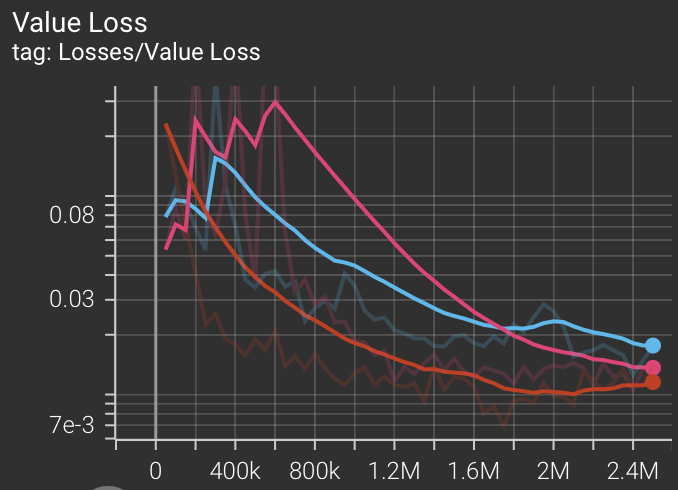
\includegraphics[width=0.99\columnwidth]{Chapter3/HU/layers_loss.png}\par
\caption{
$2$ layers (red) achieves lower $3$ layers (blue) and $1$ layer (pink)
}
\label{fig:la_loss}
\end{multicols}
\end{figure*}

The results for the different number of layers for the NN model in our agent is depicted in Figure \ref{fig:la_cumreward} and \ref{fig:la_loss}. It clearly shows that our model with just $2$ layers outperform all other choices. This could be because $3$ layers requires more data to train as it fails to generalise and over-fits. While the $1$ layer model is under-fitted as it does not have enough capacity to learn the tasks.

\subsection{Batch and Buffer size}
\begin{figure*}
\centering
\begin{multicols}{3}
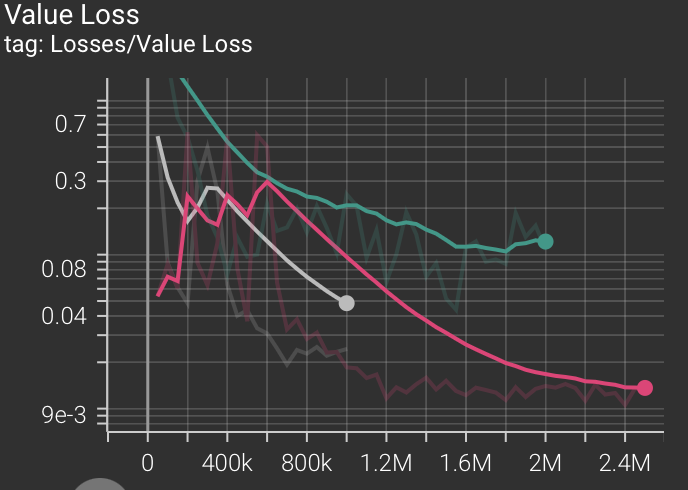
\includegraphics[width=0.99\columnwidth]{Chapter3/Batch/batch_value.png}\par
\caption{Green shows the model training with size of $32$ batch size which under performs when compared to Grey and Pink's batch size of $512$. While Pink's buffer size of $2048$ performs better than Grey's $4096$ over the long run. }
\label{fig:batch_value}

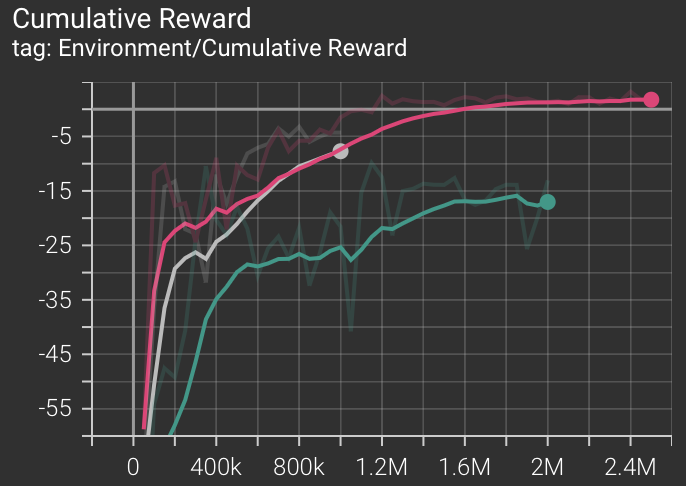
\includegraphics[width=0.99\linewidth]{Chapter3/Batch/batch_cum.png}\par
\caption{Green's performance is very weak compared to the others. Similarly Pink's buffer size of $2048$ achieves higher rewards than Grey's $4096$ over the long run.}
\label{fig:batch_cumreward}

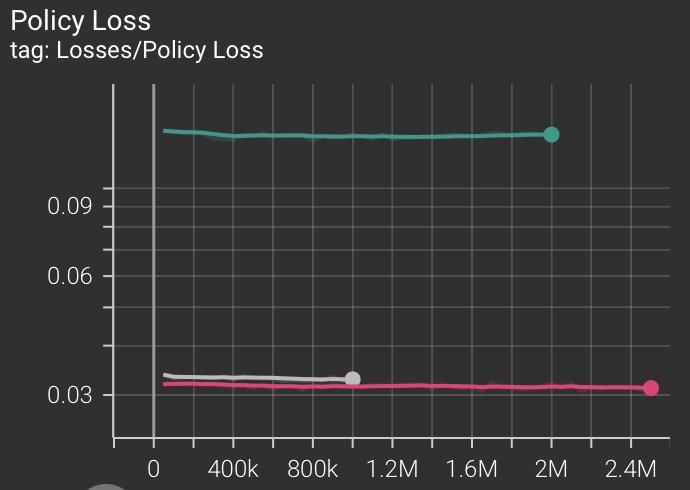
\includegraphics[width=0.99\columnwidth]{Chapter3/Batch/batch_policy_loss.png}\par
\caption{
Green's policy loss is much higher compared to the other two.
}
\label{fig:batch_policy}
\end{multicols}
\end{figure*}

Batch size is the number of experiences used for one iteration of a gradient descent update. According to unity, if the agent has continuous action space batch size should be between $32$ and $512$. While if the agent has discrete action space, then the value to should be between $512$ and $5120$. The batch size is also limited by the machine's memory size. On the other hand, buffer size corresponds to how many experiences (agent observations, actions and rewards obtained) should be collected before any learning or updating of the model. 

Since the agent tank can decide on the degree of angel to turn at any time, in this sense, the agent has a continuous action space. However, in deciding to shoot or not, the agent tank has a discrete action space, since its a Boolean logic. Hence, intuitively the buffer should be somewhere around $512$. Additionally, the number of possible agent experience should not be too large as the environment should be relatively simple as the agent is not moving. This is evident from the results depicted in Figure. \ref{fig:batch_cumreward}, \ref{fig:batch_policy}, \ref{fig:batch_value}. Batch size cannot be small, otherwise results will be very bad. On the other hand, buffer size cannot be too large. Although, in short run, models trained with buffer size of $4096$ and $2048$ achieves similar results and trends in the same direction. As agents learns more, models with the smaller buffer size performs better and achieves better results faster. As observed from the pink and grey graph in Figure. \ref{fig:batch_cumreward}, \ref{fig:batch_policy}, \ref{fig:batch_value}.


\subsection{Exploit or Explore}
Most reinforcement learning algorithms from a classic dilemma, to exploit or to explore. Exploring means that the agent will act as randomly as possible in an attempt to find more ways that could earn higher expected rewards. In Unity, under the 'reward signal', there is a extrinsic module as well as a curiosity module which enables us to configure parameters to instruct when the agent should explore when extrinsic rewards are sparse. Where extrinsic rewards refers to rewards gained from the environment. Exploitation is a scenario where the agent would maximise its expected rewards based on its current understanding of the environment. Both of which should be carefully balanced, such that the rewards agent gets from the environment (i.e. killing an enemy tank or sheltering a friendly tank) do not overwhelm the curiosity reward (i.e. how surprised the agent is). For example, if the agent is not curious and have realised that it could gain rewards by killing tank. If curiosity is not strong enough, it may not realise that it will gain rewards if the agent shelters a friendly, and may instead follow its current knowledge of simply killing all tanks.

Both of these signals have the parameters strength $\mathbb{S}$ and gamma $\gamma$. Strength represents the constant factor which is used as a multiplier to the raw reward. The $\mathbb{S}_{extrinsic} \in \mathbb{R}^+$ and $\mathbb{S}_{curiosity} \in [0.001, 0.1]$ is set at recommended values of $1.0$ and $0.1$ respectively. $\gamma$ represents the discount factor which put more weights to the recent rewards. This helps the agent to think how far into the future it should care with respect to the expected rewards. Similarly, both $\gamma_{extrinsic} \in [0.8 , 0.995]$ and $\gamma_{curiosity} \in [0.8, 0.995]$ is set to recommended value of $0.99$. 

\subsection{Time Horizon, learning rate, epsilon}
\begin{figure*}
\centering
\begin{multicols}{2}
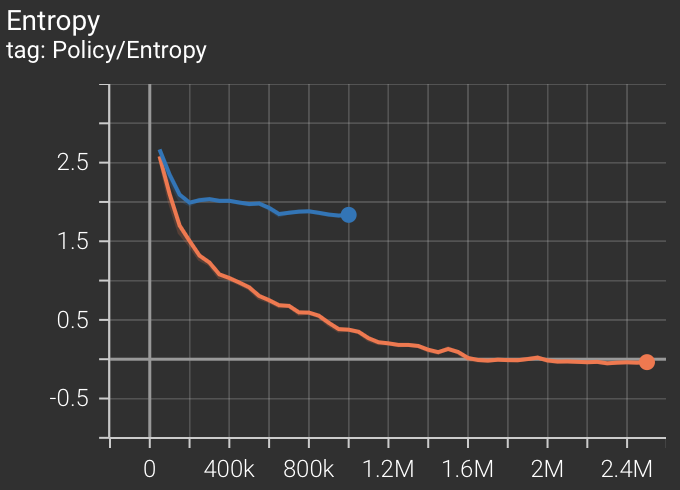
\includegraphics[width=0.99\columnwidth]{Chapter3/Epsilon/epsi_Entropy.png}\par
\caption{Higher epsilon value of 0.3 (orange) achieves lower entropy than lower epsilon value of 0.1 (blue).}
\label{fig:eps_entropy}

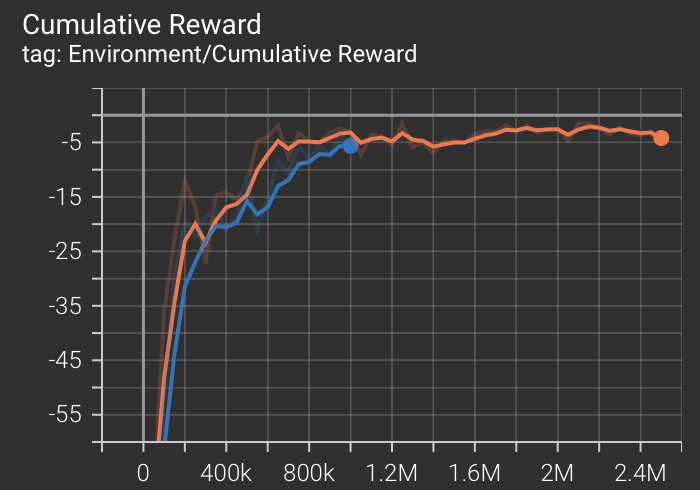
\includegraphics[width=0.99\linewidth]{Chapter3/Epsilon/eps_cum.png}\par
\caption{Higher epsilon value of 0.3 (orange) achieves slightly higher rewards than lower epsilon value of 0.1 (blue).}
\label{fig:eps_cumrewards}

\end{multicols}
\end{figure*}


\begin{figure*}
\centering
\begin{multicols}{2}
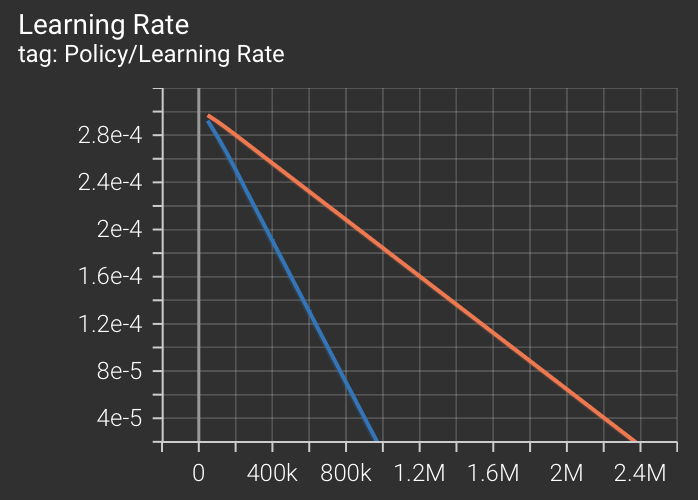
\includegraphics[width=0.99\columnwidth]{Chapter3/Epsilon/Learning_rate.png}\par
\caption{Higher epsilon value of 0.3 (orange) reduces learning rate slower than lower epsilon value of 0.1 (blue).}
\label{fig:learning_rate}

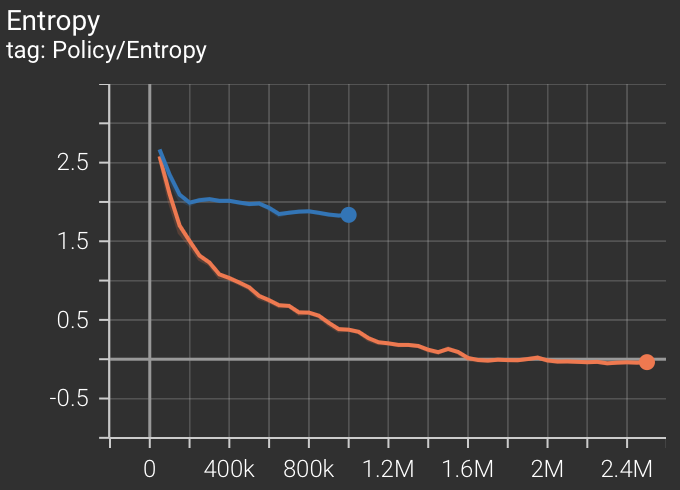
\includegraphics[width=0.99\linewidth]{Chapter3/Epsilon/epsi_Entropy.png}\par
\caption{Higher epsilon value of 0.3 (orange) is reduced over time to help stabilize training when time horizons shortens.}
\label{fig:eps}

\end{multicols}
\end{figure*}

The learning rate, $\eta$ affects the speed of the training process. Lower learning rate corresponds to smaller update step for each gradient descent. In other words, $\eta$ will affect how much the policy changes. Although this results in slower convergence rate but it allows the agent to converge more in a more stable fashion. Intuitively, a lower learning rate should reflect longer time horizon to allow the agent to have more time and episodes to learn. However, to experiment more efficiently, training time horizon has been truncated and the initial results and trends will be compared first (as seen from the result figures). Finally, the most promising parameters will be used for a full run to evaluate for final model. 

$\epsilon \in [0.1, 0.3]$ represents the tolerable threshold of divergence between the old and new policies when performing gradient descent updates. Simply put, $\epsilon$ limits to the amount of policy change. Smaller $\epsilon$ will result in more stable updates, however, it will slow down the training process too.  From Figure. \ref{fig:eps_entropy},
the orange graph representing $\epsilon=0.3$ achieves lower entropy than the blue graph representing $\epsilon=0.1$. This shows that higher $\epsilon$ is able to help the model make less random decision. However, both trends similar in terms of the reward they are able to achieve. This is depicted in Figure \ref{fig:eps_cumrewards}. In definite terms, the orange graph performs slightly better compared to the blue one. It is also noted that $\epsilon$ decreases over time and larger $\epsilon$ results in less steeper decline (both linearly)in $\eta$ as seen in Figures. \ref{fig:eps} and \ref{fig:learning_rate} respectively.


\subsection{Final Model}

\begin{figure}[t]
    \centering
    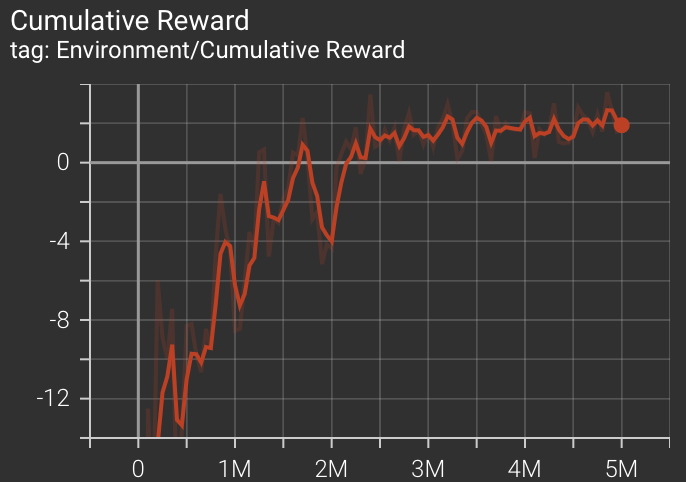
\includegraphics[width=0.99\columnwidth, height=0.7\columnwidth]{Chapter3/Final/Final_Cum.png}\par
    \caption{Agent is able to achieve very high reward scores, with highest reaching 3.57.}
    \label{fig:final_cumreward}
\end{figure}
\begin{figure*}
\centering
\begin{multicols}{2}
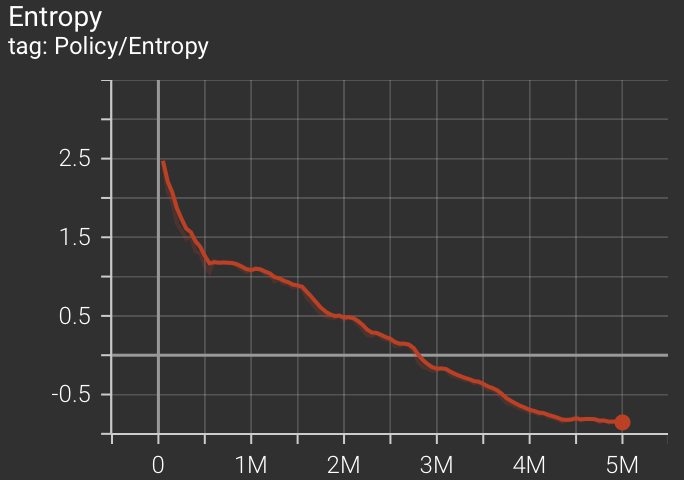
\includegraphics[width=0.99\columnwidth]{Chapter3/Final/Final_Entropy.png}\par
\caption{Combining all the best parameters results in very low entropy achieved, value of -0.8 is acheived .}
\label{fig:final_entropy}

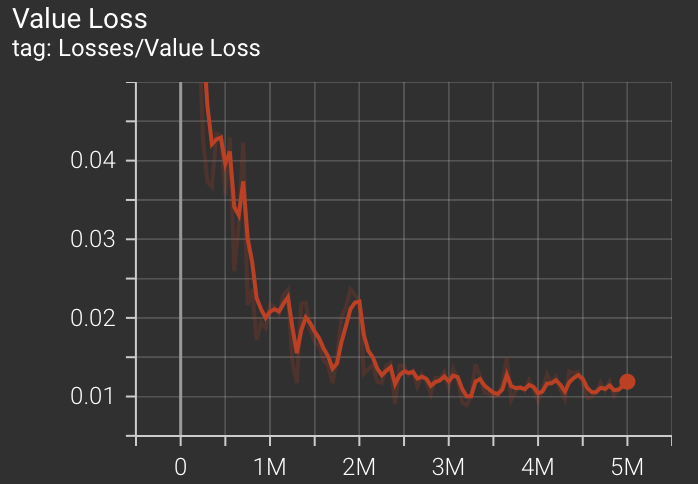
\includegraphics[width=0.99\columnwidth]{Chapter3/Final/Final_Value_loss.png}\par
\caption{
Model achieves very small losses, with lowest value of less than 0.01.
}
\label{fig:final_valueLoss}
\end{multicols}
\end{figure*}


The final variables used are summarized in Table \ref{tab:sym1}. The model is able to achieve excellent result as depicted in Figures. \ref{fig:final_cumreward}, \ref{fig:final_entropy}, \ref{fig:final_valueLoss}. This agent was able to hit above cumulative reward score of 3, way above the 0.625 mark that we loosely estimated. As expected, the agent did perform well as it will be shown in the video. 

\begin{table}[ht]
%\renewcommand{\arraystretch}{1.3}
\caption{Symbols}
\centering
\resizebox{1\linewidth}{!}{
\begin{tabularx}{1\linewidth} { X X }
\toprule
\textbf{Parameter} & \textbf{Values}  \\
\midrule
batch size & 512 \\
buffer size & 2048 \\
learning rate, $\eta$ & 0.0003 \\
beta, $\beta$ & 0.001 \\
epsilon, $\epsilon$ &  0.2 \\
lambda, $\lambda$ & 0.95 \\
epoch & 50 \\
learning rate schedule & linear \\
hidden units, HU & 256 \\
number of layers & 2 \\
$\mathbb{S}_{extrinsic}$ & 1.0\\ 
$\mathbb{S}_{curiosity}$ & 0.1  \\
$\gamma_{extrinsic}$ / $\gamma_{curiosity}$  & 0.99 \\
max steps & 5000000 \\
\bottomrule
\end{tabularx}
}
\label{tab:sym1}
\end{table}



%=== Conclusion ===

\chapter{Conclusion}


\section{Difficulty}
Since almost no coding is used to build the DRL, the difficulty actually lies in the optimization of hyperparameters used. Each training session takes atleast 8 hours, and results are not guaranteed each time hyperparameters are tuned. To counter this problem, some training are truncated once bad trends are shown. However, it is also good to note that for example in Figure \ref{fig:beta_valueLoss}, even though this set of parameters resulted in poor training for the first three million steps, in the last million steps it showed promising results and the loss starts to drop. Hence, initial trend may not necessarily tell the whole story, and prudent steps have to be taken to improve agent's performance. The amount of rewards also play a strong role in helping the agent to learn.

\section{Future Works}
In the future, the game can be extended into multi-agent mode where both enemies and turret are controlled by DRL algorithms. In fact, as an example, we could do an experiment where enemies adopt SAC algorithm and turret adopt PPO algorithm to evaluate which algorithm perform better with which kind of scenario. More interesting dynamics can be added in, such as power ups where if agent shoots a box, the agent would have unlimited attack range or super turning speed for a limited amount of time. Basically, relaxation of restrictions.  This could increase the level of difficulty for the agent.

\section{Project Summary}
In this report, we went through of the design of a unity-based DRL prototype game and the process of building the DRL agent as well as the analysis of its performance.




%==== ENDING PART ===
  \clearpage
  \pagenumbering{arabic}%
  \renewcommand{\thepage}{R-\arabic{page}}
\lhead{}
\rhead{References}
\printbibliography[title={References}]

%=================================
\newpage
\appendix
\renewcommand{\chapname}{Appendix }
\pretocmd{\chapter}{%
  \clearpage
  \pagenumbering{arabic}%
  \renewcommand*{\thepage}{\thechapter-\arabic{page}}%
}{}{}
\rhead{Appendix \thechapter}
\lhead{Source Information}
\include{Appendix/A}
%==== END OF ALL ===
\end{document}
